\newpage
\subsection{Integrators}
\label{sec:integrators}
In Mitsuba, the different rendering techniques are collectively referred to as
\emph{integrators}, since they perform integration over a high-dimensional
space. Each integrator represents a specific approach for solving
the light transport equation---usually favored in certain scenarios, but
at the same time affected by its own set of intrinsic limitations.
Therefore, it is important to carefully select an integrator based on
user-specified accuracy requirements and properties of the scene to be
rendered.

In Mitsuba's XML description language, a single integrator
is usually instantiated by declaring it at the top level within the
scene, e.g.
\begin{xml}
<scene version=$\MtsVer$>
    <!-- Instantiate a unidirectional path tracer,
         which renders paths up to a depth of 5 -->
    <integrator type="path">
        <integer name="maxDepth" value="5"/>
    </integrator>

    <!-- Some geometry to be rendered -->
    <shape type="sphere">
        <bsdf type="diffuse"/>
    </shape>
</scene>
\end{xml}

This section gives a brief overview of the available choices
along with their parameters.

\subsubsection*{Choosing an integrator}
Due to the large number of integrators in Mitsuba, the decision of which
one is suitable may seem daunting. Assuming that the goal is to solve
the full light transport equation without approximations, a few integrators
(\pluginref{ao}, \pluginref{direct}, \pluginref{vpl})
can already be ruled out. The adjoint particle tracer \pluginref{ptracer} is
also rarely used.

The following ``algorithm'' may help to decide amongst the remaining ones:
\begin{enumerate}
\item Try rendering the scene with an appropriate path tracer. If this gives the desired result, stop.

Mitsuba currently comes with three path tracer variations that target different setups: If your
scene contains no media and no surfaces with opacity masks, use the plain path tracer (\pluginref{path}).

Otherwise, use one of the volumetric path tracers (\pluginref[volpathsimple]{volpath\_simple}
or \pluginref{volpath}). The latter is preferable if the scene contains glossy surface scattering models.
\item If step 1 produced poor (i.e. noisy and slowly converging) results, try
the bidirectional path tracer (\pluginref{bdpt}).
\item If steps 1 and 2 failed, the scene contains a relatively difficult lighting setup, potentially
including interaction with complex materials.
In many cases, these difficulties can be greatly ameliorated by running a ``metropolized'' version
of a path tracer. This is implemented in the Primary Sample Space MLT (\pluginref{pssmlt}) plugin.
\item If none of the above worked, the remaining options are to try a photon mapping-type
method (\pluginref{photonmapper}, \pluginref{ppm}, \pluginref{sppm}) or a path-space MLT
method (\pluginref{mlt}, \pluginref{erpt}).
\end{enumerate}

\subsubsection*{Path depth}
\begin{figure}[htb!]
\centering
\hfill
\smallrendering{Max. depth = 1}{pathdepth-1}
\smallrendering{Max. depth = 2}{pathdepth-2}
\smallrendering{Max. depth = 3}{pathdepth-3}
\smallrendering{Max. depth = $\infty$}{pathdepth-all}
\caption{
    \label{fig:pathdepths}
    These Cornell box renderings demonstrate the visual
    effect of a maximum path depth. As the paths
    are allowed to grow longer, the color saturation
    increases due to multiple scattering interactions
    with the colored surfaces. At the same time, the
    computation time increases.
}
\end{figure}

Almost all integrators use the concept of \emph{path depth}.
Here, a path refers to a chain of scattering events that
starts at the light source and ends at the eye or sensor.
It is often useful to limit the path depth (\figref{pathdepths})
when rendering scenes for preview purposes, since this reduces the amount
of computation that is necessary per pixel. Furthermore, such renderings
usually converge faster and therefore need fewer samples per pixel.
When reference-quality is desired, one should always leave the path
depth unlimited.

\begin{figure}[h!]
\centering
\vspace{-5mm}
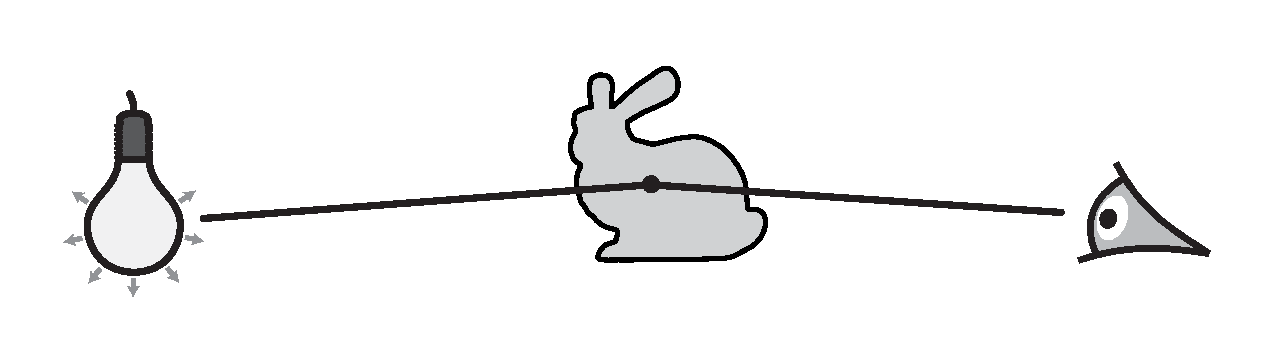
\includegraphics[width=10cm]{images/path_explanation.pdf}
\vspace{-5mm}
\caption{
    \label{fig:path-explanation}
    A ray of emitted light is scattered by an object and subsequently
    reaches the eye/sensor.
    In Mitsuba, this is a \emph{depth-2} path, since it has two edges.
}
\end{figure}
Mitsuba counts depths starting at $1$, which correspond to
visible light sources (i.e. a path that starts at the light
source and ends at the eye or sensor without any scattering
interaction in between).
A depth-$2$ path (also known as ``direct illumination'') includes
a single scattering event (\figref{path-explanation}).

\subsubsection*{Progressive versus non-progressive}
Some of the rendering techniques in Mitsuba are \emph{progressive}.
What this means is that they display a rough preview, which improves over time.
Leaving them running indefinitely will continually reduce noise (in unbiased algorithms
such as Metropolis Light Transport) or noise and bias (in biased
rendering techniques such as Progressive Photon Mapping).
\newpage
\subsubsection*{Hiding directly visible emitters}
\label{sec:hideemitters}
Several rendering algorithms in Mitsuba have a feature to hide directly
visible light sources (e.g. environment maps or area lights). While not
particularly realistic, this feature is often convenient to remove a background
from a rendering so that it can be pasted into a differently-colored document.

Note that only directly visible emitters can be hidden using this feature---a
reflection on a shiny surface will be unaffected. To perform the kind of
compositing shown in Figure~\ref{fig:hideemitters}, it is also necessary to
enable the alpha channel in the scene's film instance (Section~\ref{sec:films}).

\renderings{
  \unframedrendering{Daylit smoke rendered with \code{hideEmitters} set to \code{false}
     (the default setting)}{integrator_volpath_normal}
     \unframedrendering{Rendered with \code{hideEmitters} set to \code{true} and alpha-composited
      onto a white background.}{integrator_volpath_hideemitters}
      \caption{\label{fig:hideemitters}An example application of the \code{hideEmitters} parameter
    together with alpha blending}
}
